%!TEX root = ../main.tex

\section{Вычислительный эксперимент}

\subsection{Параметры модели, краевые условия}

Была создана программа, реализующая в рамках разностной схе\forcehyphenation мы \eqref{sch:borders},~\eqref{sch:transition},~\eqref{sch:time_step_min_max} перечисленные ранее алгоритмы адаптации временного шага: по фазовому полю \eqref{sch:time_step_phi}, по энергии \eqref{sch:time_step_energy} и по устойчивости \eqref{sch:time_step_stability}.

Будем использовать параметры модели, отражающие реальный физический эксперимент: см. табл. \ref{tab:parameters}. Часть параметров ($| \nabla \Phi|$, $\epsilon_0$) являются полноценными физическими величинами, часть ($\Gamma$, $m$) могут быть подобраны для согласования модели с результатами эксперимента. Чертой отделены параметры, которые либо происходят из связанных с диффузной границей допущений ($l$, $\delta$), либо описывают расчетную сетку.

\begin{table}[!t]
\captionsetup{justification=raggedright,singlelinecheck=false}
\caption[]{Параметры модели в расчете}
\centering
\begin{tabular}{|l|c|l|}
	\hline
	Название & Параметр & Значение \\
	\hline
	электрическое напряжение		& $|\nabla \Phi|$	& $5.625 \cdot 10^6 \; \unitV / \unitm$							\\
	энергия роста ед. длины канала	& $\Gamma$			& $8.118 \cdot 10^{-10} \; \unitJ / \unitm$						\\
	диэлектрическая проницаемость	& $\epsilon_0$		& $2.301 \cdot 10^{-11} \; \unitC^2 / (\unitJ \cdot \unitm)$	\\
	подвижность						& $m$				& $12 \; \unitm^3 / (\unitJ \cdot \units)$						\\
	\hline
	характерная толщина границы		& $l$ 				& $1.5 \cdot 10^{-6} \; \unitm$									\\
	регуляризующий параметр 		& $\delta$			& $10^{-3}$														\\
	размер образца					& $W$				& $3.2 \cdot 10^{-5} \; \unitm$									\\
	продолжительность опыта			& $T$				& $2 \cdot 10^{-3} \; \units$									\\
	шаг по пространству				& $h$				& $5 \cdot 10^{-7} \; \unitm$									\\
	минимальный шаг по времени		& $\tau_{min}$		& $10^{-10} \; \units$											\\
	максимальный шаг по времени		& $\tau_{max}$		& $\leqslant 6.42 \cdot 10^{-6} \; \units$						\\
	\hline
\end{tabular}
\label{tab:parameters}
\end{table}

Заметим, что, таким образом, число узлов сетки по пространству $N_x = 64$, по времени -- $312 \leqslant N_t \leqslant 2 \cdot 10^7$.

Зададим следующие краевые условия:
\begin{gather}
	\phi(0, t) = \phi(W, t) = 1, \qquad \phi(x, 0) = \phi_0(x),
	\label{exp:border} \\
	\phi_0(x) = \begin{cases}
		1 - 0.025 \cdot \left( 1 + \cos \left[ \cfrac{\pi}{0.08} \left( \cfrac{x}{W} - \half \right) \right] \right) \text{ при } \cfrac{x}{W} \in [0.42, 0.58]; \\
		1 \text{ иначе}.
	\end{cases}
	\nonumber
\end{gather}
Функция $\phi_0(x)$ отлична от $1$ в небольшой области вокруг $x = W / 2$, где <<прогибается>> как один период $\cos$, достигая минимума $\phi = 0.95$.


\subsection{Структура сетки с переменным шагом по времени}

Итак, на каждой итерации по времени используется своя величина шага~$\tau_k$. Таким образом, расчетная сетка теряет регулярность по времени, и сравнение разных решений по сеточной норме становится нетривиальной задачей. Введем у нерегулярной сетки определенную структуру, в которой сконцентрируем всю сложность вопроса, избегая при этом использования сеточной интерполяции для результатов расчетов.

Пусть $N = N_{t, max} = T / \tau_{min} \in \Natural$, то есть временной промежуток $[0, T]$ разбит $N + 1$ узлом на $N$ равных отрезков длиной $\tau_{min}$ каждый. Над этим разбиением введем структуру <<типа дерева отрезков>>. Говоря формально, будем считать допустимыми лишь разбиения вида $D = (0, p_1 \tau_{min}, p_2 \tau_{min}, \dots$, $p_{m - 1} \tau_{min}, N \tau_{min})$, где $p_k \in \Natural_0$, $k = \overline{0, m}$, $p_k$ строго возрастают, $L_k = p_k - p_{k - 1} \hm = 2^{s_k}$, $s_k \in \Natural_0$, и к тому же $p_{k - 1} \divby L_k$.

Описанная структура замечательна тем, что если из любых двух допустимых разбиений $D_1$ и $D_2$ выбрать по интервалу, то либо эти интервалы не пересекаются, либо совпадают, либо один строго вложен в другой. Следовательно, любые два соседних узла объемлющего разбиения $D = D_1 \cap D_2$ (пересечение в смысле множеств) соседствуют также в $D_1$ или в $D_2$ -- в таком ключе $D$ оптимально.

При адаптации шага по времени в разностной схеме \eqref{sch:borders},~\eqref{sch:transition},~\eqref{sch:time_step_min_max} на итерации $k$ будем использовать не рассчитываемое $\tau_k$ напрямую, а максимальное $\tau_k' = 2^s \tau_{min} \leqslant \tau_k$, $s \in \Natural_0$ к тому же допустимое описанным разбиением <<типа дерева отрезков>> временного промежутка $T$ на $N$ отрезков, а именно:
\begin{gather*}
	p_0 = 0, \quad p_k = p_{k - 1} + 2^{s_k} \leqslant N, s_k \in \Natural_0; \\
	\tau_k' = 2^{s_k} \cdot \tau_{min} \leqslant \tau_k, \quad p_{k - 1} \divby 2^{s_k}; \\
	s_k \to \max.
\end{gather*}

Для сравнения по равномерной норме $\enorm_{C, h}$ двух сеточных решений~$\phi_1$ и~$\phi_2$ на разбиениях $D_1$ и $D_2$ соответственно ограничим их оба на объемлющем разбиении $D = D_1 \cap D_2$.


\subsection{Результаты расчетов}

На рис. \ref{fig:solution_basic} изображен результат расчета с параметрами из табл. \ref{tab:parameters} и краевыми условиями \eqref{exp:border} без адаптации шага по времени. Видно, как из малого начального возмущения фазового поля $\phi$ постепенно растет канал электрического пробоя. В момент времени $t \approx 1.82 \cdot 10^{-3}$ в точке $x = W / 2$ фазовое поле $\phi$  становится мало отличимо от $0$ -- происходит <<пробой насквозь>>. Обратим внимание, что значение фазового поля упало от $\phi \approx 0.6$ до $\phi \approx 0$ менее чем за время $10^{-5}$, то есть $0.5 \%$ от всего времени эксперимента. Далее канал пробоя растет в толщину примерно с постоянной скоростью.

\begin{figure}[!t]
	\centering
	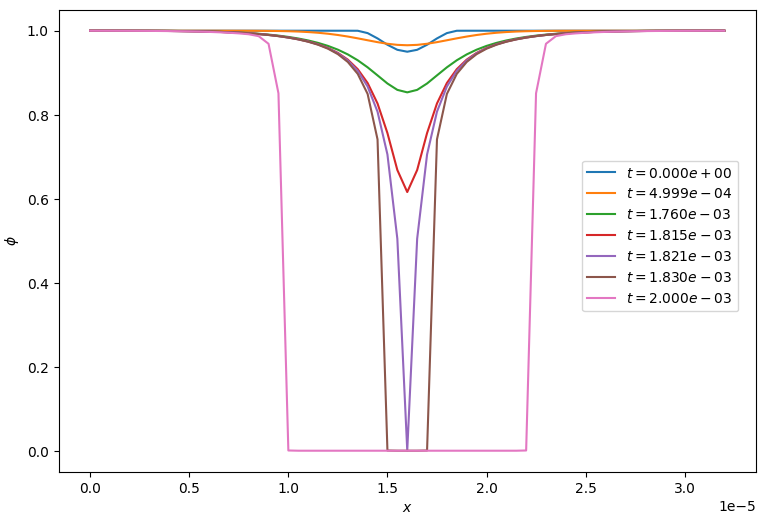
\includegraphics[width=\textwidth]{figures/solution_basic.png}
	\vspace{-0.8cm}
	\caption{Решение задачи (расчет без адаптации)}
	\label{fig:solution_basic}
\end{figure}